\documentclass[a4paper, 11pt]{article}
\usepackage{comment} % enables the use of multi-line comments (\ifx \fi) 
\usepackage{lipsum} %This package just generates Lorem Ipsum filler text. 
\usepackage{fullpage} % changes the margin
\usepackage{listings}
\usepackage{hyperref}
\usepackage{color}
\usepackage{graphicx}


\definecolor{mygreen}{rgb}{0,0.6,0}
\definecolor{mygray}{rgb}{0.5,0.5,0.5}
\definecolor{mymauve}{rgb}{0.58,0,0.82}

\lstset{ %
  backgroundcolor=\color{white},   % choose the background color; you must add \usepackage{color} or \usepackage{xcolor}
  basicstyle=\footnotesize,        % the size of the fonts that are used for the code
  breakatwhitespace=false,         % sets if automatic breaks should only happen at whitespace
  breaklines=true,                 % sets automatic line breaking
  captionpos=b,                    % sets the caption-position to bottom
  commentstyle=\color{mygreen},    % comment style
  deletekeywords={...},            % if you want to delete keywords from the given language
  escapeinside={\%*}{*)},          % if you want to add LaTeX within your code
  extendedchars=true,              % lets you use non-ASCII characters; for 8-bits encodings only, does not work with UTF-8
  keepspaces=true,                 % keeps spaces in text, useful for keeping indentation of code (possibly needs columns=flexible)
  keywordstyle=\color{blue},       % keyword style
  language=Octave,                 % the language of the code
  otherkeywords={*,...},           % if you want to add more keywords to the set
  numbers=none,                    % where to put the line-numbers; possible values are (none, left, right)
  numbersep=5pt,                   % how far the line-numbers are from the code
  numberstyle=\tiny\color{mygray}, % the style that is used for the line-numbers
  rulecolor=\color{black},         % if not set, the frame-color may be changed on line-breaks within not-black text (e.g. comments (green here))
  showspaces=false,                % show spaces everywhere adding particular underscores; it overrides 'showstringspaces'
  showstringspaces=false,          % underline spaces within strings only
  showtabs=false,                  % show tabs within strings adding particular underscores
  stepnumber=2,                    % the step between two line-numbers. If it's 1, each line will be numbered
  stringstyle=\color{mymauve},     % string literal style
  tabsize=3,	                   % sets default tabsize to 2 spaces
}


\begin{document}
%Header-Make sure you update this information!!!!
\noindent
\large\textbf{CA650 Software Process Quality}  \hfill \textbf{Anthony Troy} \\
\normalsize XUnit Report \hfill Date: 25/2/2016

\section*{Report Requirements}
Using any XUnit-style framework, implement a class for creating and adding integers to a Stack with a corresponding test suite. Typically you should have \lstinline$create$,  \lstinline$push$,  \lstinline$pop$ and  \lstinline$isEmpty$ methods.

\section*{Attachments}
Convenient browsing of the discussed source code in this report is available through the following GitHub repository: \href{https://github.com/full-of-foo/pystack}{full-of-foo/pystack}. The involved files of note
are as follows:
	\begin{itemize}
		\item \textit{pystack/\_\_init\_\_.py}
		\item \textit{pystack/exc.py} (package exception declarations) 
		\item \textit{pystack/stack.py} (stack implementation module)
		\item \textit{tests/\_\_init\_\_.py}
		\item \textit{tests/fixtures.py} (test fixture module)
		\item \textit{tests/test\_stack.py} (test suite for the stack)
		\item \textit{report/report.pdf}
		\item \textit{report/report.tex} (LaTeX file for this report)
		\item \textit{setup.py} (python package setup module)
		\item \textit{test\_requirements.txt} (listing for test requirement packages)
		\item \textit{tox.ini} (test runner configuration file)
		\item \textit{circle.yml} (continuous integration service configuration file) 
\end{itemize}	
\section*{Stack Implementation}
Under Python 3.5, we implement our  list-based stack as follows:
\\
\lstinputlisting[language=Python, firstline=0]{../pystack/stack.py}


\section*{Test Suite Implementation}
Using \lstinline$unittest$, Python's native XUnit framework, we implement our stack test suite as follows:
\\
\lstinputlisting[language=Python, firstline=0]{../tests/test_stack.py}

\section*{Test Runner Implementation}
Leveraging \lstinline$tox$, an open-source packaging and test runner framework for Python, we implement the following test run tasks:
\lstinputlisting[language=sh, lastline=19]{../tox.ini}

\section*{Test Suite Execution}
\noindent As entailed above, our default task simply runs all \lstinline$unittest$ test suites in the current package. The output of such a run is as follows:

\\
\lstinputlisting[language=sh]{tox_out.txt}

\section*{Local Coverage Execution}
Our second task, named ``coverage", executes a popular Python line coverage tool against our source code. The output of this coverage run is as follows:

\\
\lstinputlisting[language=sh]{cov_out.txt}

\section*{Automated Testing Implementation}
Our \lstinline$pystack$ project avails of a continuous integration service named CircleCI. The service will build and execute our test suite upon the pushing of a candidate build to a given remote GitHub branch. One can browse 
these builds at \href{https://circleci.com/gh/full-of-foo/pystack}{circleci.com/gh/full-of-foo/pystack}. Our configuration for the service is as follows:
\\
\lstinputlisting[language=yaml,lastline=11]{../circle.yml}

\\
In a production scenario there might be an extra step in this configuration that deploys our \lstinline$pystack$ package to a server given that the build, and in turn tests, have passed. We have defined
a new run task that will execute our test suite and also generate a HTML report of our line coverage which is persisted by the CircleCI service per build. 
By doing so during the build process we can ensure that coverage in the project will be maintained, as builds not reaching 100\% coverage will fail. This ``circle" run task is as follows:
\\
\lstinputlisting[language=sh, firstline=20]{../tox.ini}

\newpage
\section*{Automated Test Execution}
Upon pushing a commit to our remote GitHub master branch we  trigger a new build on CircleCI. Some example output from this successful build is as follows:
\\
\\
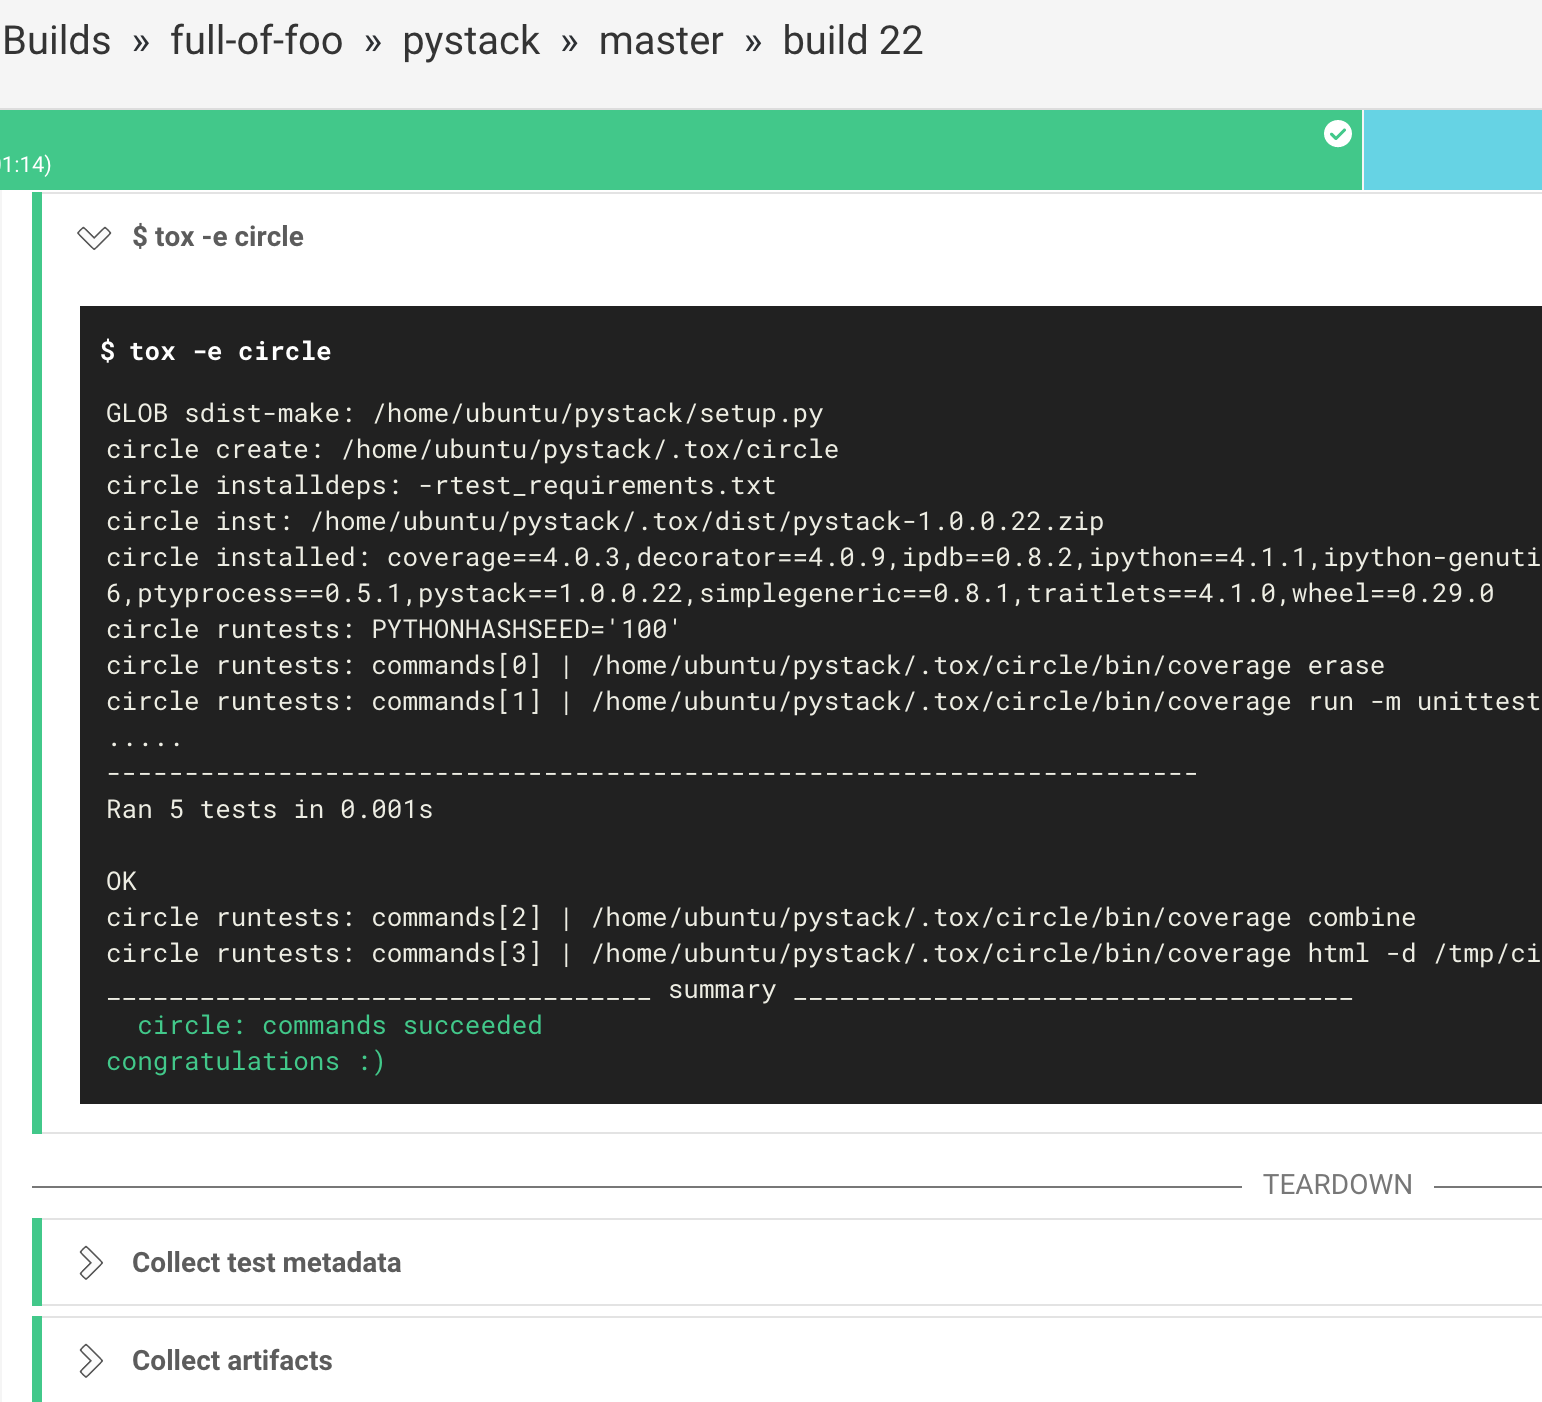
\includegraphics[scale=0.58]{circle}
\\
\\
When this successful build completes CircleCI makes our build artefacts available. These include a  \lstinline$coverage/index.html$ file which allows us browse the coverage report for 
the given build:
\\
\\
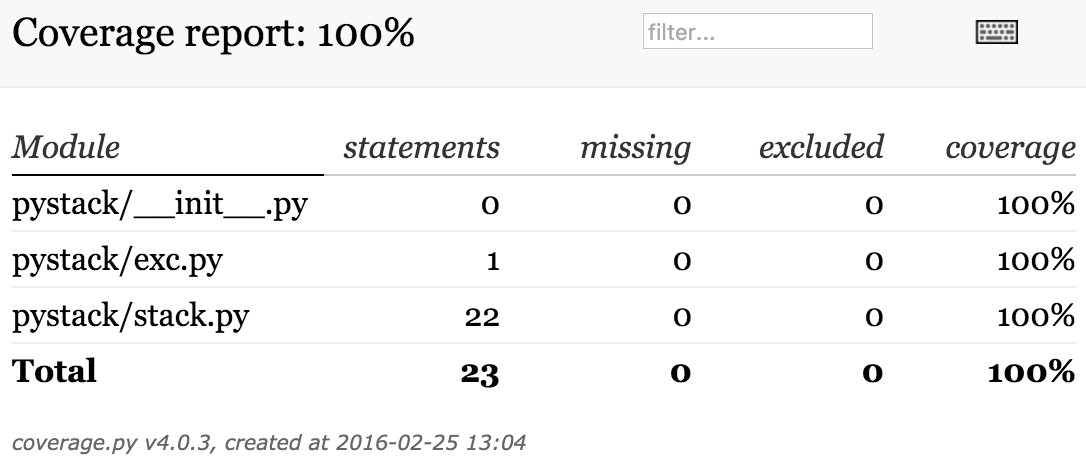
\includegraphics[scale=0.6]{cov}
 


\end{document}
